%mainfile: master.tex
\chapter{Teorier og metoder}
\label{chap:teorier_og_metoder}
I dette afsnit bliver der set på de relavante teorier og metoder der bliver anvendt til problematikken ved Nytrov. Herunder bliver der givet en introduktion til hver emne, før det bliver præsenteret i rapporten.

\section{Anvendelse af Shared Space}
\label{sec:shared_space}
I dette underafsnit bliver Shared Space teorien og hvad der karakterisere Shared Space beskrevet, samt hvor og hvorledes det anvendes.
\subsection{Hvor anvendes Shared Space?}
\label{sub:hvor_anvendes_share_space}
Shared space anvendes oftest i områder med kryds, strækninger fra sted til sted, samt sammenhængende områder, såsom bycentre med smalle gader. Derudover anvendes shared space også i mindre landsbyer, tættere bymæssig bebyggelse, hvor der er blandede erhverv, og bymidter. Betingelsen for hvordan de ovennævnte områder fungerer som ‘shared space’, er ved, at der er lav hastighed, begrænset trafikmængder og balance mellem de forskellige trafikantgrupper, hvor ingen bestemt trafikantgruppe dominerer over de andre trafikgrupper. Shared space fungerer også som en alternativ vej, som afvikler trafikmængden af biler og cykler. Derfor anvendes shared space ikke ved trafikveje, cykelruter og bustrafik områder, da den ikke prioriterer en bestemt trafikgruppe i området. %(https://da.glosbe.com/da/sv/t%C3%A6ttere%20bebygget%20omr%C3%A5de 17/11-2015) og (http://vejregler.lovportaler.dk/showdoc.aspx?t=%2fV1%2fNavigation%2fTillidsmandssystemer%2fVejregler%2fAnlaegsplanlaegning%2fTrafikarealer+by%2fVejgeometri+i+byomrader%2f&docId=vd-shared-space-full 17/11-2015)
\subsection{Trafikmængder og hastigheder}
\label{sub:Trafikmaengder_og_hastgheder}
Det anbefales, at shared space anvendes ved trafikmængder på maks. 3.000- 4.000 motorkøretøjer pr. døgn. I tysk litteratur anbefales 4.000 motorkøretøjer, hvorimod engelsk litteratur anbefaler 2.000 motorkøretøjer med en hastighed på 30 km/t. Holland har områder, som er udformet med shared space, der afvikler 15.000 motorkøretøjer pr. døgn. Dette medvirker, at trafikken med store mængder trafik køretøjer fylder, og får fodgængere til at være ekstra opmærksomme på at krydse vejene. På Skvallertorget i den svenske by Norrköping har man erfaret, at mængden af fodgængere skal udgøre halvdelen, mere end de forventede antal biler. Nogenlunde samme antal cykler og biler skal være til stede, for at skabe balance i trafikken. Det anbefales, at kørende trafik i et shared space område bør udformes med en hastighed på 15-20km/t, hvilket svarer til en meget lav hastighed. %(http://vejregler.lovportaler.dk/showdoc.aspx?t=%2fV1%2fNavigation%2fTillidsmandssystemer%2fVejregler%2fAnlaegsplanlaegning%2fTrafikarealer+by%2fVejgeometri+i+byomrader%2f&docId=vd-shared-space-full 17/11-2015)
\subsection{Ens eller dobbeltrettet}
\label{sub:ens_eller_dobbeltrettet}
Shared space er udformet som dobbeltrettede gader. Dette resulterer i en bedre adgang til området uden at der skal foretages nogle omveje for trafikken, hvorimod ensrettet vej vil prioritere den ene kørselsretning. Dette medfører en højere hastighed og tavler, som er i strid med shared space princippet, der ligger til grund for at reducere hastigheden og afmærkningerne. I den anledning bør shared space altid være dobbeltrettet, da den også skal tage hensyn til cykler, der cykler i hver sin retning. %(http://vejregler.lovportaler.dk/showdoc.aspx?t=%2fV1%2fNavigation%2fTillidsmandssystemer%2fVejregler%2fAnlaegsplanlaegning%2fTrafikarealer+by%2fVejgeometri+i+byomrader%2f&docId=vd-shared-space-full 17/11-2015)

\subsection{Busser og parkering}
\label{sub:Busser_og_parkering}
Det anbefales ikke at føre bustrafik gennem et shared space område, men i særlige tilfælde kan det ske under korte strækninger.  Da hastigheden i shared space område er lav, kan bussen risikere at blive bremset eller forsinket af krydsende fodgængere. City- og servicebuslinjer kan føres gennem shared space områder, dog tager ruteplanlægningen højde for, at busserne forventer lav hastighed i området.
I et shared space område bør parkeringen være begrænset, og der skal være afmærkede båse. Derudover skal et shared space område tilbyde passende cykel parkeringsfaciliteter. %(http://vejregler.lovportaler.dk/showdoc.aspx?t=%2fV1%2fNavigation%2fTillidsmandssystemer%2fVejregler%2fAnlaegsplanlaegning%2fTrafikarealer+by%2fVejgeometri+i+byomrader%2f&docId=vd-shared-space-full 17/11-2015)

\subsection{Eksempler på Shared Space anvendelse}
\label{sub:eks_shared_space}
DER KOMMER BILLEDER - ENDNU IKKE LAVET


\section{Observationsmetoder}
\label{sec:observationsmetoder}
I følgende underafsnit bliver der set på observationsmetoder samt bliver der givet definition på hvad en konflikt egentlig er.
\subsection{Definition af konflikt}
\label{sub:def_konflikt}
Begrebet konflikt, er et meget vidt begreb og dækker indenfor flere fagområder,1 men i denne rapport, bliver der nærmere undersøgt for begrebet indenfor vej og trafik. Som umiddelbart vil man definere konflikt, som sammenstød mellem to trafikkanter, men dog udelukker den svenske trafikteknik denne påstand. Den svenske trafikteknik beskriver en konflikt mellem to trafikkanter, som har kollisionskurs og vil kolligere, hvis en af trafikkanterne ikke foretager sig en pludselig reaktion for, at forhindre kollisionen.2 Det vil sige, at sålænge et uheld (sammenstød) kan undgås af mindst en af trafikanterne, så vil der være tale om en konflikt. Ved hjælp af den svenske trafikteknik, kan man dele en konflikt i flere grad. De forskellige konfliktgrad er defineret som, alvorlige konflikter, mindre alvorlige konflikter og potentielle konflikter, som også kan ses på figur 4.1 :
 \begin{figure}[htbp]
   \label{fig:indellingkonflikter}
   \centering
   \begin{adjustbox}{max width=\textwidth}
     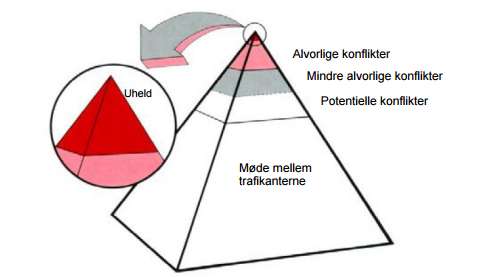
\includegraphics{billederogfigur/konflikt.png} %http://www.trafitec.dk/sites/default/files/publications/konfliktteknikstudier%20i%20kbh%20bykryds.pdf
  \end{adjustbox}
   \caption{Inddeling af konflikter}
 \end{figure}
\newpage
 En konfliktgrad bestemmes ved hjælp af TU-værdi. TU-værdi er defineret som Tid til Ulykke eller også kaldes det TA, altså Time to Accident. Metoden bag bestemmelse af TU-værdien gøres ved hjælp af følgende formel:
 \begin{equation}
  TU=d/V
\end{equation}

Formelen fortæller om forholdet mellem distancen, til det potentielle punkt i en kollision og hastigheden når en af trafikanterne undviger uheldet. Heraf kan der ved hjælp af figur 4.2, ses om konfliktet er alvorlig eller ej.
~\\\\

\begin{figure}[htbp]
  \label{fig:tugraf}
  \centering
  \begin{adjustbox}{max width=\textwidth}
    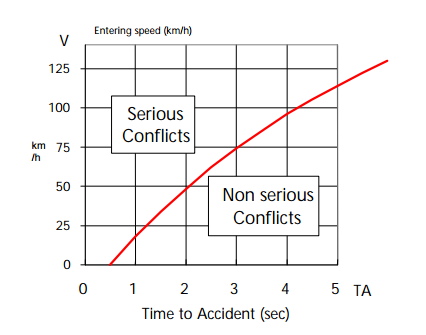
\includegraphics[scale=0.6]{billederogfigur/tugraf.png} %http://www.tft.lth.se/fileadmin/tft/video_in_traffic/Swedish_conflict_technique.pdf
 \end{adjustbox}
  \caption{TU-graf}
\end{figure}

Som der kan ses på figuren, så er alvorligheden af en konflikt afhængig af både distance samt hastighed, dog har hastighed en større rolle, i tilfælde af hastigheden er høj.
På baggrund af TU- tabellen kan der ses, at en TU værdi over 0.5 ses som ikke alvorlig konflikt, hvorimod en TU værdi under ca. 0.5, vil være en alvorlig konflikt.

I næste afsnit vil der blive ses på, nogle observationsmetoder, som skal anvendes for identificere konflikter ved området i Nytorv.
~\\
\subsection{Adfærdsstudier}
\label{sub:adfaerdsstudie}

Når	man	vil	observere	nogle	konflikter	mellem	to	eller	flere	forskellige
trafikantgrupper,	må	man	lave	nogle	antagelser	om,	hvad	der	egentlig	vil	føre	til	en
konflikt.	Man	må	altså	på	forhånd	opstille	nogle	hypoteser,	som	man	via	nogle
undersøgelsesspørgsmål,	kan	bruge	til	at	forudse	nogle	formåede	konflikter	mellem
nogle	bestemte	trafikantgrupper.	Baggrunden	for	denne	måde	at	undersøge
konflikter	på ligger	i,	at	man	sjældent	vil	have	mulighed	for	at	observere	selve
konflikterne	eller	uheldene,	da	det	ikke	vil	være	dagligdag	på	det	givne
observationssted.	I	denne	undersøgelse	om	fodgængernes	tryghed	på	Nytorv,	vil
man altså	ikke	på	observationsdagen	formode,	at	man direkte	vil	observere en
alvorlig	konflikt	eller	et	uheld	mellem	en	fodgænger	og	en	cyklist.	Måden	man
derimod	vil	kunne	undersøge	de	opstillede	hypoteser	på	og	bygge	sine	spørgsmål	op
omkring,	vil	være	at	bruge	en	evalueringsmetode,	hvor	man	kigger	på
adfærdsstudier.i Her	fokuserer	man	på	den	typiske	normale	adfærd	på	sit
observationssted, og	det	skal	så	underbygge	hypoteserne. Hele	ideen	bag	denne
evalueringsmetode	er	at	”forcere	indhentningen	af	data”	(samme	kilde),	altså	at
forudsige	data	som	belæg	for	sine	antagelser.
I	denne	undersøgelse	vil	adfærdsregistreringen	blive	bygget	op	omkring	figur	(Figur
3	i	det	udleverede	litteratur),	hvor	fokus	ligger	på	dels	ankomsten	mellem
fodgængere	og	cyklister	og	dels	ankomsten	mellem	fodgængere	og	biler på
observationsstedet. Udgangspunktet	herfra	er	så	at	undersøge,	om	der	i	samtidige
ankomster	er	et	tidligt	samspil	eller	et	sent	samspil	mellem	de	to	trafikanter.
Herefter	vurdere,	om	hændelsen ud	fra	de	to	parametre	gik	godt,	om	der	opstod	en
konflikt	eller	der	decideret	skete	et	uheld.	Hypotesen	er	så,	at	hvis	antallet	af	tidlige
samspil	stiger	og	antallet	af	sene	samspil	falder,	så	vil	trafiksikkerheden,	og	derved
trygheden,	blive	forøget.
\begin{figure}[htbp]
  \label{fig:adfreg}
  \centering
  \begin{adjustbox}{max width=\textwidth}
    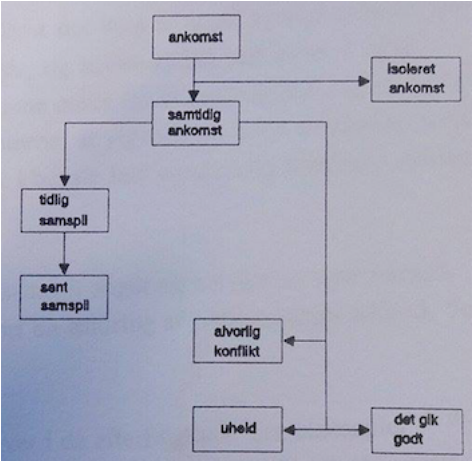
\includegraphics[scale=0.7]{billederogfigur/adfaerdsreg.png} %papir fra vejledern
 \end{adjustbox}
  \caption{Adfærdsregistrering}
\end{figure}
\\\
\subsection{Adfærdsregistrering}
\label{sub:adfregis}

Dette	afsnit	er	inspireret	af	kilden	Konfliktteknik	og	adfærdsstudier.
For	at	kunne	registrere	den	typiske	normale	adfærd	ud	fra	figuren,	er	det	vigtigt	at
definere	de	forskellige	begreber.
I	tabel	(??)	kan	man	se	en	opdeling	af	de	forskellige	begreber,	en	definition	af	dem
og	en	optælling	af	de	forskellige	tilfælde.	Alle	tilfældene	finder	sted	i	en	samtidig
ankomst,	da	der	i	en	isoleret	ankomst	ikke	vil	kunne	opstå	en	konflikt	mellem	to
parter.	En	samtidig	ankomst	er	i	vores	undersøgelse	defineret	som	cyklisten	eller
bilens	ankomst	”til	konfliktpunktet	mindre	end	2.5	sek	efter	eller	mindre	end		1.0	sek	før	fodgængeren.” (kilde	udleveret	litteratur)	Ligeledes	skal	cyklen	eller	bilen
ikke	være	påvirket	af	andre	parter.	De	skal	altså	være	fritkørende.	Definitionen	på
en	fritkørende	bil	eller	cyklist	vil	være,	at	de	ikke	er	styret	af	nogle	forankørende
eller	tæt	bagvedkørende,	som	eventuelt	ville	kunne	påvirke fart	og	opmærksomhed.
\\\\
\begin{figure}[htbp]
  \label{fig:adfregtabel}
  \centering
  \begin{adjustbox}{max width=\textwidth}
    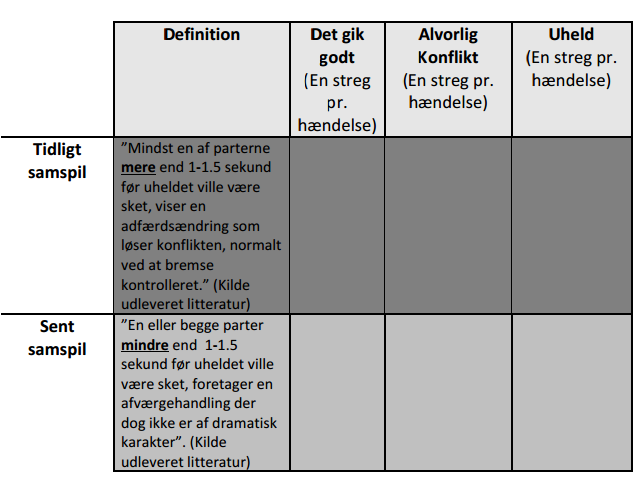
\includegraphics{billederogfigur/obstabel.png} %papir fra vejledern
 \end{adjustbox}
  \caption{Adfærdsregistreringstabel}
\end{figure}
\\\\
\textbf{"Det	gik	godt"} er	defineret	som	en	passering	af	konfliktpunktet,	hvor	situationen
har	været	under	kontrol	og	der	har	været	afstand	mellem	parterne.
8
\\\\
\textbf{"Alvorlig konflikt"}	er	defineret	ud	af	en	afværgehandling,	som	ville	have	ført	til	en
kollision	mellem	to	parter. Afværgehandlingen	sker	inden	for	1-1.5	sekund	før	den
mulige	kollision%(udleveret	litteratur).
Konfliktgraden kan også defineres udfra TA-værdien.
\\\\
\textbf{"Uheld"} er	defineret	ved	en	kollision	mellem	to	parter.



\section{Trafiktællinger}
\label{sec:trafiktaellinger}

Dette afsnit er inspireret af kilden %http://vej08.vd.dk/mastra/mastradok/dok/TrafiktaellingerPlanUdfoerEfterb.pdf
\\
Trafiktællinger udføres til mange formål. Det gælder alt fra at kontrollere den overordnede vejplanlægning
til at undersøge klagesager om for høje trafik hastigheder. Trafiktællinger bruges bl.a. til at finde løsninger
til opgaver omhandlende trafiksikkerhed, kapacitet og miljøforhold, samt statistikker over trafikudviklingen
og hastigheden af vejnettet. Man kan foretager trafiktællinger manuelt eller ved brug af maskiner.
Manuelle tællinger fungerer ved at personer registrere trafikken på det pågældende sted, ofte ved hjælp af
tælleblokke, håndtællere eller håndterminaler. (Mere om manuelle tællinger \cref{sec:manueltaelling}). Ved maskine
tælling fortages registreringerne automatisk ved brug af et tælleapparat, hvor mennesker ikke medvirker.
\subsection{Manuel Tælling}
\label{subs:manueltaelling}

Manuel tælling er som sagt, hvor det er mennesker der tæller trafikken. Manuel tælling er en god metode,
når der ønskes at kende trafikkens specifikke trafikstrømme. Et typisk forløb for manuel tælling er opbygget
op af 6 trin.
\\\\
1) Som det første skal formålet for tællingen bestemmes, samt hvilken resultat type, som ønskes af opnå.
\\\\
2) Der skal besluttes placeringen af tælleposterne, hvor der skal tages hensyn til at tælleren ikke genere
trafikken. Tællerne skal også have frit udsyn for parkerende biler, buskaser og lignende under hele
tælleperioden. Man skal derfor overveje om forholdene kan ændre sig undervejs.
\\\\
3) En af de betydelige usikkerheder ved trafiktællinger, er valget af tælleperioden. Der kan være meget stor
variation fra dag til dag og time til time, hvis man. ønsker at finde årsdøgntrafikken. Der er f.eks. stor forskel
på trafikmængden i weekenden kontra hverdage og myldertiden om morgen og eftermiddagen kontra
andre midt på dagen og om aftenen og natten. Manuelle tællinger vare typisk 4, 6 eller 12 timer og
sjældent et helt døgn.
\\\\
4) Når tælleposterne og tidspunkterne er fastlagt, bestemmes antallet af tællere til posterne, efter
trafikmængden ved stedet. Ifølge vejdirektoratet er kvaliteten af resultaterne afhænger af antal tællere. Er
tælleposterne underbemandet, vil resultaterne blive uanvendelige. Hvis man er uvidende om
trafikmængden, og dermed antallet af tæller som er nødvendige, kan man foretage en prøvetælling inden.
Der skal også bestemmes valget af tælleudstyr. Ved mindre trafikmængder kan der anvendes blyant og papir, ved større trafikmængder anvendes ofte håndtællere, håndterminaler eller tællepulte.
\begin{figure}[htbp]
  \label{fig:taellingstabel}
  \centering
  \begin{adjustbox}{max width=\textwidth}
    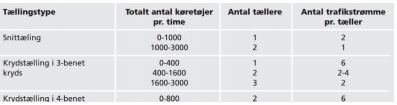
\includegraphics{billederogfigur/Taellingstabel.png} %papir fra vejledern
 \end{adjustbox}
  \caption{Viser antallet af erfarne tæller pr. trafikant i timen}
\end{figure}
\\
En håndtæller består typisk af et apparat med en knap, som tæller 1 frem, hver gang der trykkes, og en anden knap som nulstiller apparatet igen. Håndterminaler –og pulte, er et mere avanceret værktøj. Apparatet kan tælle flere trafikgrupper af gangen, eller hvilken retning trafikken kommer fra, på både snitlængde og på krydstællinger.

\begin{figure}[htbp]
  \label{fig:krydstaelling}
  \centering
  \begin{adjustbox}{max width=\textwidth}
    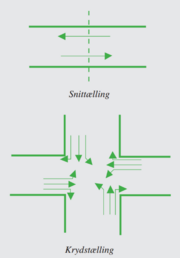
\includegraphics{billederogfigur/krydstaelling.png} %papir fra vejledern
 \end{adjustbox}
  \caption{Viser eksempel på krydstælling og snittælling}
\end{figure}
~\\\\
5) Inden tællerne begynder, er det vigtigt at de er sat sig ind i overstående bestemmelser for tælleforløbet, således der ikke opstår tvivler undervejs. Ligeledes udarbejdes et tælleskema inden tællingen påbegyndes.
~\\\\
6) Resultatbehandling af tællingen.
